%What are epicardial leads
\glspl{cied} systems refer to cardiac implantable electronic devices, including pacemakers, \glspl{icd}, \gls{crt} devices, and implanted rhythm monitors. These are advanced medical devices used to monitor and regulate heart rhythm disorders. Out of these components, cardiac leads are a type of very thin,  $\sim$4 to 5 F (French gauge, meaning 1.3 to 1.7 mm), electrical wire that connects a pulse generator to the heart enabling two-way communication between them. Their main functions include, monitoring, pacing, and defibrillation.

%Epicardial leads design %Types
%how do they differ from transvenous leads?

%Physical Description of the leads
Cardiac lead types are differentiated by three main things, placement in the heart, polarity, and their fixation mechanism. The later is the method used to secure the lead tip to the heart tissue to prevent movement.
In practice, Figure \ref{fig:epivstransLeads} shows the two types of leads that are used, epicardial leads which are implanted directly on the epicardium (the outer surface of the heart) and transvenous leads, inserted through the veins and positioned inside the heart's chambers, making contact with the endocardium (the inner lining of the heart). Both are prone to complications such as fracture, infection, and venous obstruction (transvenous only) requiring complex extraction procedures \cite{Defaye_Europace_2023, Russo_JACC_AUC_2025}.

\begin{figure}[h!]
	\centering
	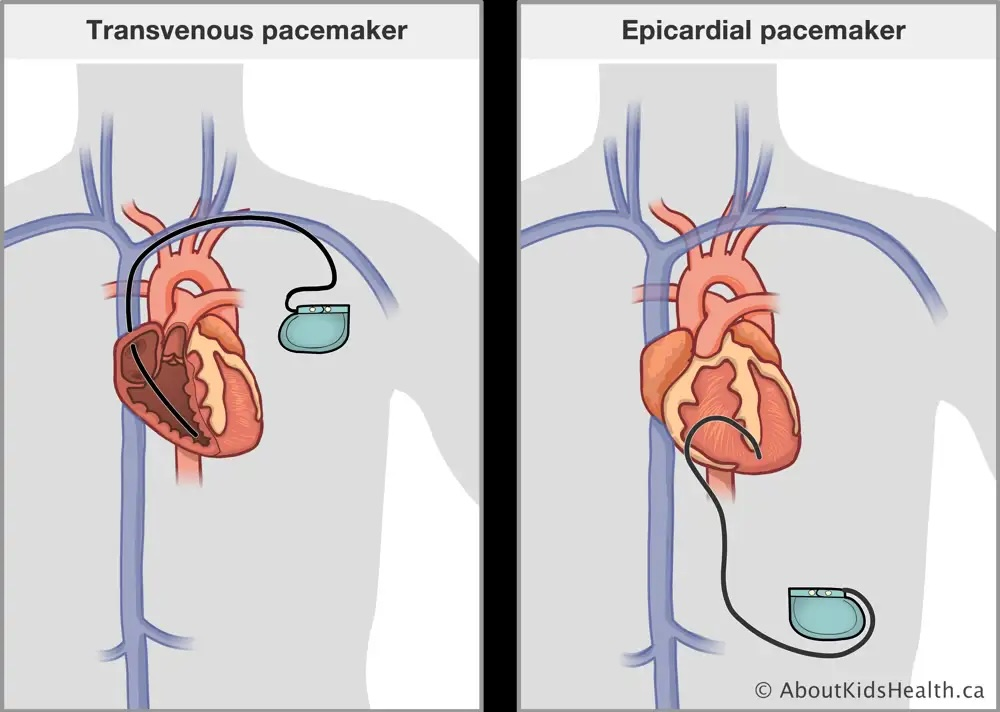
\includegraphics[width=0.45\columnwidth]{Assets/epivstransLeads.jpeg}
	 \caption[Comparison of transvenous vs epicardial lead]{Comparison of transvenous vs epicardial lead placement in pacemakers. Reproduced in accordance with the AboutKidsHealth Image Use Policy 
	 	\cite{AboutKids_Pacemaker2009}, \copyright~2004--2026 AboutKidsHealth..}
	 \label{fig:epivstransLeads}
\end{figure}

The position of leads is an important distinction. Clinically, these leads are indicated for different populations and diagnostics therefore carry a variety of management decisions (leaving vs. extracting) and different complications (percutaneous lead extraction or transvenous lead extraction) \cite{meier2024, Murayama:2008aa}. Physically, the type of tissue contact differs between lead placements and carries distinct mechanical and thermal consequences. For instance, transvenous leads are surrounded by blood, which can cool the lead and reduce its effective heating capacity.

Beyond thermal effects, any induced displacement force or vibration on transvenous leads may be modified by surrounding blood flow, vessel-wall contact, and tissue fixation, which can constrain lead motion and alter force transmission. Epicardial leads, by contrast, are mechanically constrained differently. They are exposed on the outer surface of the heart, anchored by suture or screw fixation directly onto the epicardium, so any mechanically induced force acts at that fixation interface \cite{Haggani_CCPDRT_ch4_2011}. The fixation mechanisms for each lead type are shown in Figure \ref{fig:leadFixation}. 

\begin{figure}[hb!]
	\centering
	\subfloat[\label{fig:tvleadFixation}]{
	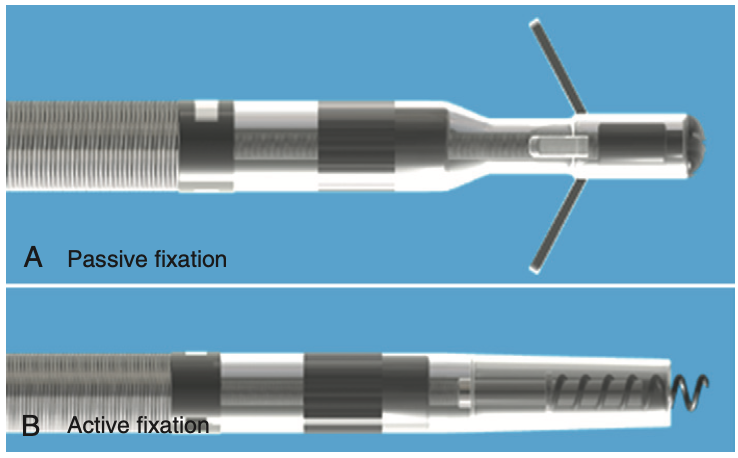
\includegraphics[width=0.55\textwidth]{Assets/activevspassiveFixation.png}
	}
	\hfill
	\subfloat[\label{fig:epileadFixation}]{
		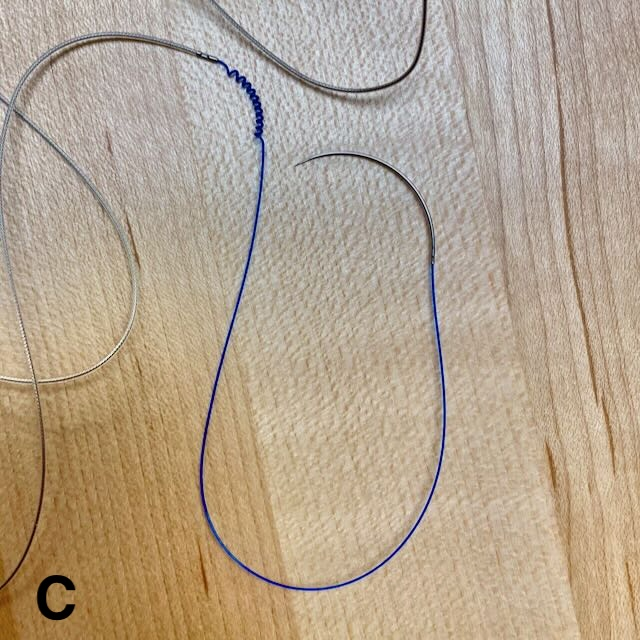
\includegraphics[width=0.38\textwidth]{Assets/epileadReal.jpeg}
	}
	
	\caption[Lead fixation variations in pacing leads]{Lead fixation variations in pacing leads.
		(A) Passive-fixation leads rely on flexible tines that anchor within myocardial trabeculae. (B) Active-fixation leads employ a retractable helix that screws into the myocardium. 
		Reprinted from \textit{Clinical Cardiac Pacing, Defibrillation, and Resynchronization Therapy}, Haqqani et al., p. 133, Copyright (2011), with permission from Elsevier \cite{Haggani_CCPDRT_ch4_2011}.
		(C) Medtronic STREAMLINE\textsuperscript{\texttrademark}~6492 unipolar epicardial lead with suture needle at the proximal end followed by a blue fixation coil. 
		}
	\label{fig:leadFixation}
\end{figure}

%Fixation distiguishes the two types
Epicardial leads are most commonly fixed by suturing directly onto the tissue, Figure \ref{fig:epileadFixation} shows a Medtronic STREAMLINE\textsuperscript{\texttrademark}~6492 unipolar epicardial lead with one end a swaged-on suture needle. Other mechanisms include screwing an active-fixation helix into the myocardium, shown in Figure \ref{fig:tvleadFixation} bottom panel. Transvenous leads are placed internally and secured using either passive-fixation tines that grip the heart's trabecular muscle bundles or an active-fixation helix, as shown in Figure \ref{fig:tvleadFixation} \cite{Haggani_CCPDRT_ch4_2011}.

%What are the main design variations?
%Polarity
Within epicardial leads, design may vary, including lead polarity and body structure. Figure \ref{fig:uni-bipo-comparison} shows the distinction between unipolar and bipolar configurations in terms of electrode placement and the resulting current pathways during cardiac stimulation. Unipolar leads contain a single conductor and one electrode (the cathode) is in contact with the heart. Bipolar leads contain two conductors that connect to two electrodes on the lead itself, a tip electrode (cathode) and a ring electrode (anode).

\begin{figure}[hbt!]
	\centering
	%\subfloat[Unipolar vs. bipolar epicardial lead configuration.\label{fig:uni-bi}]{
		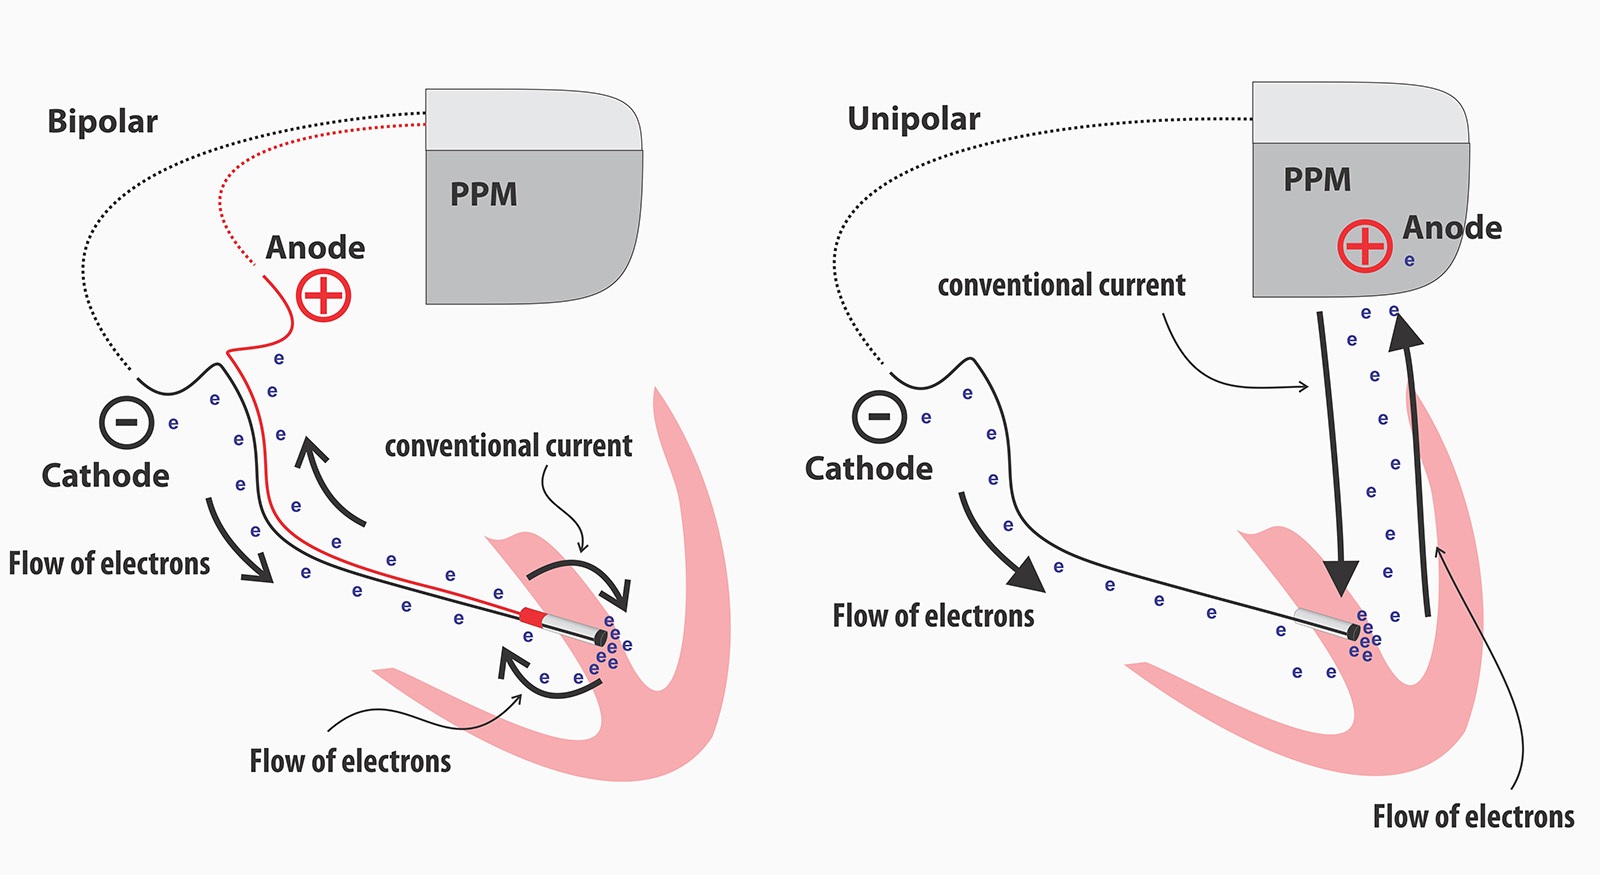
\includegraphics[width=0.55\textwidth]{Assets/uni-bi.jpg}
	%}
	%\hfill
	%\subfloat[Relative electrode positioning of unipolar and bipolar epicardial leads.\label{fig:bipo_uniPo}]{
		%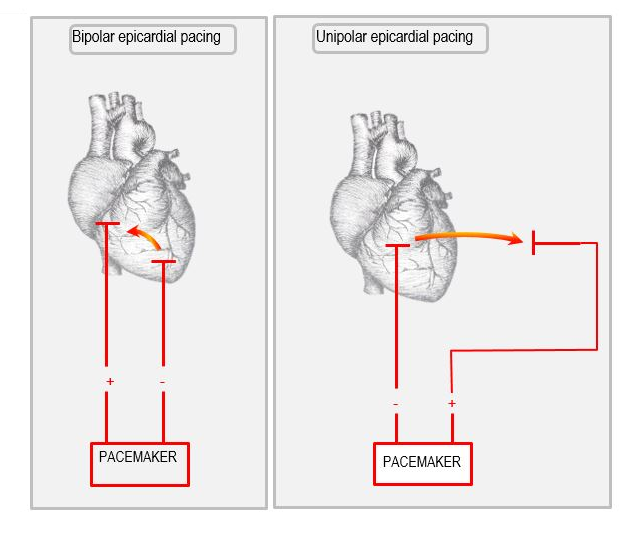
\includegraphics[width=0.48\textwidth]{Assets/bipo_uniPo-placement-cropped.png}}
	
	\caption[Comparison of unipolar and bipolar epicardial pacing leads]{Comparison of unipolar and bipolar epicardial pacing leads using a schematic of the heart's ventricle. The current flows in different pathways on each case, Reprinted from \cite{HowToPace_Basics_2023} 
		under CC BY-NC-ND 4.0.}
	\label{fig:uni-bipo-comparison}
\end{figure}

% and composition
Moreover, Bipolar leads exhibit further structural variation in their body design. As shown in Fig.~\ref{fig:leadDesign}, coaxial design features an inner coil conductor nested within an outer coil conductor, each wrapped in a separate insulation. Co-radial designs consist of a single coil containing two parallel, intertwined conductor strands, each individually insulated \cite{Haggani_CCPDRT_ch4_2011}. 

\begin{figure}[hbt!]
	\centering
%	\subfloat[Lead fixation mechanisms.\label{fig:leadFixation}]{
	%	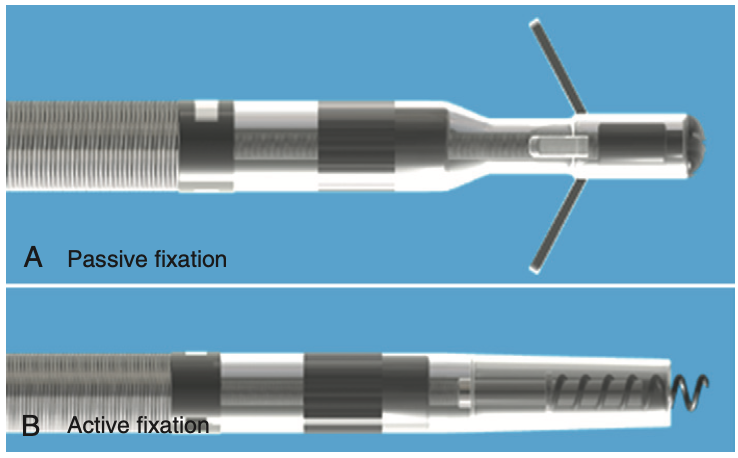
\includegraphics[width=0.48\textwidth]{Assets/activevspassiveFixation.png}
%	}
%	\hfill
%	\subfloat[Coaxial and coradial lead body design.\label{fig:leadDesign}]{
		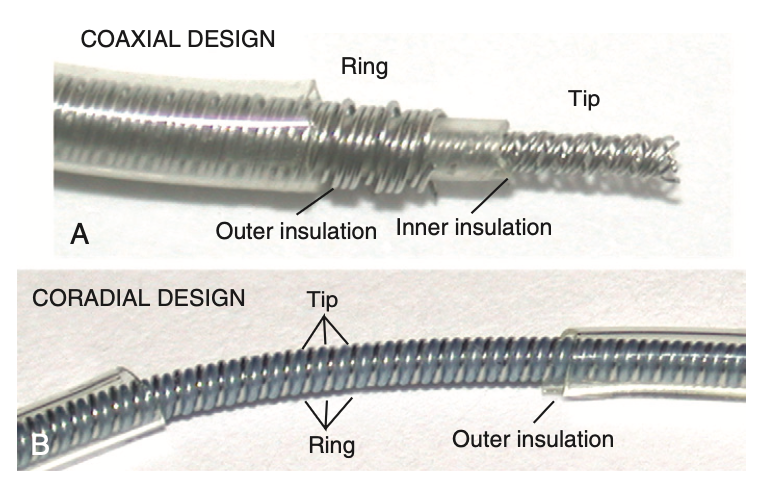
\includegraphics[width=0.45\textwidth]{Assets/CoaxialvsCoradial.png}
	%}
	
	\caption[Body design variations in pacing bipolar leads]{Body design variations in pacing bipolar leads.
		Coaxial designs use two nested coil conductors with separate insulation layers, whereas co-radial designs incorporate parallel, intertwined conductors within a shared lumen. 
		Reprinted from \textit{Clinical Cardiac Pacing, Defibrillation, and Resynchronization Therapy}, Haqqani et al., p. 133, Copyright (2011), with permission from Elsevier \cite{Haggani_CCPDRT_ch4_2011}.}
	\label{fig:leadDesign}
\end{figure}

Another important distinction is the clinical use of the epicardial lead, i.e. permanent vs. temporary leads. Permanent leads are relatively uncommon, implanted by surgeons, and primarily indicated in pediatric patients with complex congenital heart disease \cite{mriquestions_epicardial_pacing_leads}. In contrast, temporary epicardial leads are routinely placed after open-heart surgery manage arrhythmia that might arise in the postoperative period\cite{mriquestions_epicardial_pacing_leads,reade2007}. Once the patient is rhythmically stable, these wires are manually removed. However, if resistance is encountered during extraction, they may be clipped at the skin and allowed to retract, resulting in retained wire fragments within the subcutaneous tissues \cite{mriquestions_epicardial_pacing_leads,Mubarak:2023aa}.

%What materials are commonly used in epicardial lead construction?
The several components of an epicardial lead are made of different materials chosen for their biocompatibility, durability, and electrical properties. Table \ref{tab:lead_material_suscept_qual_mri} summarizes the materials found on a epicardial lead and relates to its magnetic susceptibility. Electrodes are made from inert materials to minimize corrosion and inflammatory reactions over the long term. These include titanium, platinum-iridium alloys, Elgiloy (an alloy of cobalt, iron, chromium, and other metals), and vitreous carbon \cite{Haggani_CCPDRT_ch4_2011, callister2018materials}. Similarly, conductors which carry the electrical signals between the pulse generator and the electrode are commonly made out of MP-35N (alloy of nickel, cobalt, chromium, and molybdenum) \cite{Haggani_CCPDRT_ch4_2011, carpenterMP35N}. Insulation, a protective outer coating of the lead that prevents short-circuiting is made of different polymers like Silicone Rubber (Polysiloxane), Polyurethane, Fluoropolymers \cite{Haggani_CCPDRT_ch4_2011}.

\begin{table}[htbp]
	\centering
	\caption[Magnetic susceptibility of epicardial lead materials]{Qualitative magnetic susceptibility of common epicardial lead materials and their relevance for MRI safety. \cite{astmF2182,ASTM_F2503_2023,callister2018materials,carpenterMP35N}}
	\label{tab:lead_material_suscept_qual_mri}
	\resizebox{\textwidth}{!}{
		\begin{tabular}{|c|c|c|c|}
			\hline
			\textbf{Component} & \textbf{Material} & \textbf{Magnetic susceptibility} & \textbf{Relevance for MRI safety} \\
			\hline
			Electrode & Titanium & Paramagnetic & Low; minimal torque/force in MRI \\
			Electrode & Platinum–Iridium alloy & Paramagnetic & Low; generally MRI safe \\
			Electrode & Elgiloy (Co–Cr–Fe–Ni alloy) & Paramagnetic & Moderate; may experience slight translational force \\
			Electrode & Vitreous carbon & Diamagnetic & Minimal; very low MRI interaction \\
			Conductor & MP-35N & Weakly paramagnetic & Low; minimal contribution to MRI forces \\
			Insulation & Silicone rubber (polysiloxane) & Diamagnetic & Negligible; non-conductive and non-magnetic \\
			Insulation & Polyurethane & Diamagnetic & Negligible; non-magnetic \\
			Insulation & Fluoropolymer (PTFE) & Diamagnetic & Negligible; MRI inert \\
			\hline
		\end{tabular}
	}
\end{table}

%sizes
Because epicardial leads are composed of conductive and paramagnetic materials, an abandoned lead may pose a potential risk in the MR environment. Moreover, its physical dimensions influence the nature of these interactions: greater material volume increases the extent to which the lead can interact with the magnetic field.

An abandoned epicardial lead could measure full-length or fragments after being left behind \cite{vuorinen2021,schaller2021}. Some fragments are described as long as 5 cm, being 2 cm an average length. Further, longer leads are reported up to 30 cm or couple fragments adding to about 21 cm. In diameter size may be compared to standard transvenous pacing leads, that of about half a millimeter to 1.5 mm \cite{vuorinen2021}. And are typically narrower than standard transvenous leads ($\sim$5 F, $\simeq$ 1.7 mm outer diameter), often measuring between 0.5 mm and 1.5 mm.
%How do the physical dimensions (diameter, length, insulation thickness) affect mechanical and magnetic interactions?
An example of these interaction is that lead length influences \gls{rf}-induced heating through the antenna effect. Longer leads couple more strongly with the radiofrequency field, and maximum heating is expected near the resonant length  \cite{aboyewa2021,panych2018}. For translational force and torque, the total material volume is relevant as well, as both interactions scale with volume and are evaluated relative to gravitational effects. These relationships are discussed further in Section \ref{sec:concerns}.

%Which leads are we testing on? Why this leads in particular?

%current state of the institutions that recommend saferty around MRI
Finally, current institutional recommendations regarding MRI in patients with retained epicardial leads remain conservative despite evolving evidence. Major guideline bodies, including the Heart Rhythm Society (\gls{hrs}), the \gls{esc}, and the \gls{cms}, allow \gls{mri} in patients with \gls{mri}-conditional or certain legacy cardiac implantable electronic devices (\glspl{cied}), but continue to restrict or discourage imaging in patients with abandoned or epicardial leads \cite{vuorinen2021}.

At the time of the \gls{hrs} 2017 consensus there was insufficient data to comment on the safety of \gls{mri} with an abandoned cardiac lead. Afterwards, the 2021 \gls{esc} guidelines noted that while \gls{mri} is generally permitted for many \gls{cied} patients, it is not recommended for those with epicardial leads due to theoretical risks like heating. If a patient had an \gls{mri}-conditional system along with an abandoned lead, lead extender, lead remnants, fractured lead(s), or surgically implanted epicardial leads, the system was considered non–\gls{mri}-conditional leading to a case-by-case consideration for whether to image or not and in which modality \cite{schaller2021}. \gls{cms} similarly excludes abandoned or epicardial leads from coverage due to perceived insufficient safety data, even though large observational studies indicate that modern epicardial leads (implanted after 2000) may undergo \gls{mri} safely under carefully monitored conditions \cite{vuorinen2021}.

This cautious institutional stance demonstrates the need for experimental characterization of mechanical interactions between retained epicardial leads and MRI fields. This supports the rationale for the present study. By quantifying these forces under controlled laboratory conditions, the work shown in this document directly addresses whether current institutional restrictions are justified and lays the groundwork for evidence-based updates to clinical safety policies.